\chapter{Bug found in \emph{Git}}
\label{bugappend}
\begin{lstlisting}
teste$ git init
   Initialized empty Git repository in /home/smooke/Dropbox/teste/.git/
teste$ touch f
teste$ echo a > f
teste$ git add f
teste$ git commit -m 'first commit'
   [master (root-commit) dab04b9] first commit
   1 files changed, 1 insertions(+), 0 deletions(-)
   create mode 100644 f
teste$ git branch b
teste$ touch something
teste$ echo b > something
teste$ git add something
teste$ git commit -m 'something added'
   [master 9f2b8ad] something added
   1 files changed, 1 insertions(+), 0 deletions(-)
   create mode 100644 something
teste$ git rm something
   rm 'something'
teste$ mkdir something
teste$ cd something/
something $ touch f1
something $ echo c > f1
something $ cd ..
teste$ git add something/f1
teste$ git checkout b
   Switched to branch 'b'
teste$ ls
   f
teste$ git checkout master
   Switched to branch 'master'
teste$ ls
   f  something
teste$ cat something
   b
\end{lstlisting}

\label{bugappend2}

\begin{figure}[tp]
   \centering
   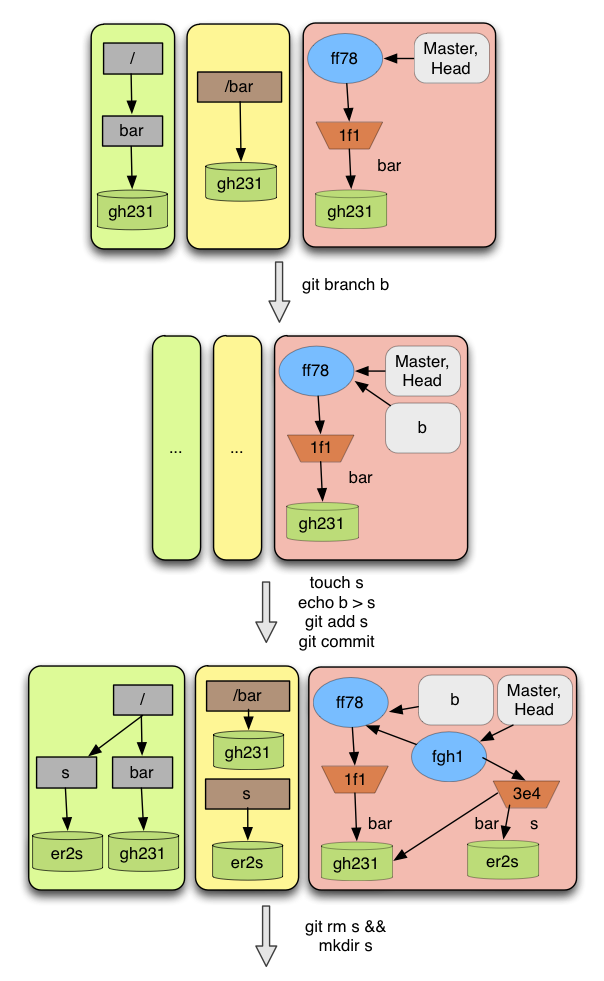
\includegraphics[width=0.8\textwidth]{images/gitbug1.png}
   \caption{Showing the git bug (part 1)}\label{fig:gitbug1}
\end{figure}
\begin{figure}[tp]
   \centering
   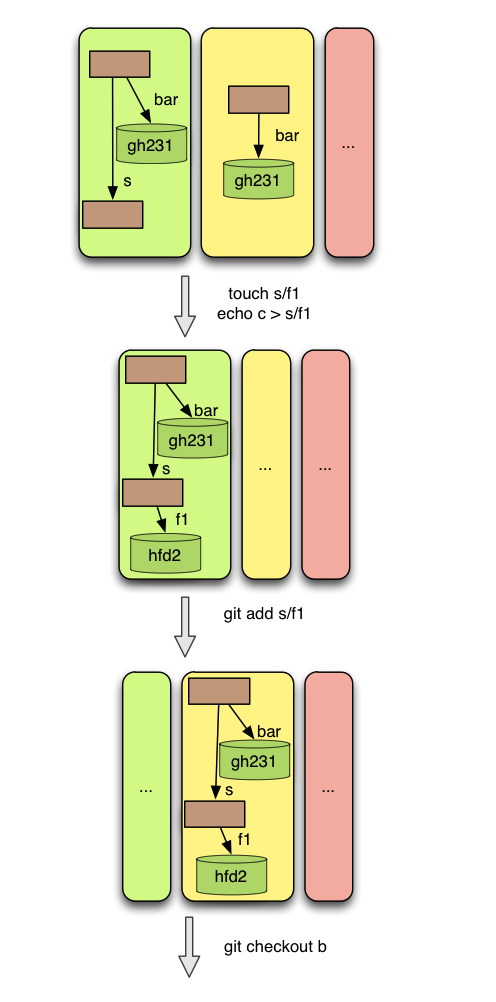
\includegraphics[width=0.5\textwidth]{images/gitbug2.png}
   \caption{Showing the git bug (part 2)}\label{fig:gitbug2}
\end{figure}
\begin{figure}[tp]
   \centering
   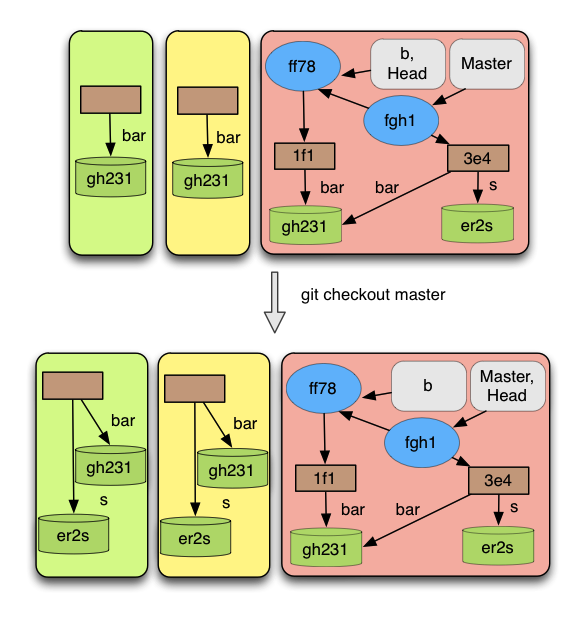
\includegraphics[width=0.8\textwidth]{images/gitbug3.png}
   \caption{Showin the git bug (part 3)}\label{fig:gitbug3}
\end{figure}

